\documentclass{article}
\usepackage{float}
\usepackage{tikz}
\usepackage{colortbl}
\usepackage{listings}
\lstloadlanguages{C}
\lstset{
language=C,
basicstyle=\ttfamily
}
\usetikzlibrary{decorations.pathreplacing}
\usetikzlibrary{positioning}
\usetikzlibrary{shapes}
\usepackage[
	pdfauthor={Buganini Q},
	pdftitle={BSDCONV}]{hyperref}
\hypersetup{
	colorlinks=false,
	pdfborder={0 0 0}
}
\title{BSDCONV}
\author{Kuan-Chung Chiu\\(buganini at gmail dot com)}
\date{}
\begin{document}
	\maketitle
	\tableofcontents
	\section{Syntax}
		\subsection{Phases \& Cascade}
			\paragraph{}
			There are three types of conversion phases defined in bsdconv: \textbf{from}, \textbf{inter}, \textbf{to}. The \textbf{from} phase takes byte sequence and decodes it into a list of code points (except for from/PASS), on the other hand, the \textbf{to} phase encodes the list of code points back to byte sequence. The \textbf{inter} phase does code point to code point mapping.
			\paragraph{}
			A basic conversion consists of \textbf{from} and \textbf{to} phases. Search of codec name is case insensitive.
			\begin{figure}[H]
				\centering
				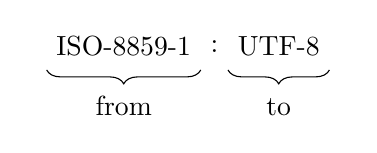
\begin{tikzpicture}[auto,node distance=0,on grid=false]

				    % Place nodes
				    \node (d0) {};
				    \node [right=of d0](from) {ISO-8859-1};
				    \node [right=of from](d1) {:};
				    \node [right=of d1] (to) {UTF-8};
				    \node [right=of to] (d2) {};
					
					\draw [decorate,decoration={brace,amplitude=5pt,raise=3mm, mirror}]
(d0)--(d1)  node  [black,midway,yshift=-1cm] { from };
				
					\draw [decorate,decoration={brace,amplitude=5pt,raise=3mm, mirror}]
(d1) -- (d2)  node [black,midway,yshift=-1cm] { to };
				
				\end{tikzpicture}
				\caption{Basic two phases conversion}
			\end{figure}
			
			\paragraph{}
			Between \textbf{from} and \textbf{to} phases, we can have an \textbf{inter} phase.
			\begin{figure}[H]
				\centering
				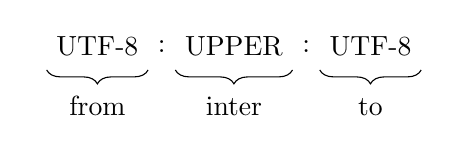
\begin{tikzpicture}[auto,node distance=0,on grid=false]			
				    % Place nodes
				    \node (d0) {};
				    \node [right=of d0](from) {UTF-8};
				    \node [right=of from](d1) {:};
				    \node [right=of d1] (inter) {UPPER};
				    \node [right=of inter](d2) {:};
				    \node [right=of d2] (to) {UTF-8};
				    \node [right=of to] (d3) {};			
					
					\draw [decorate,decoration={brace,amplitude=5pt,raise=3mm, mirror}]
	(d0) -- (d1) node [black,midway,yshift=-1cm] { from };
					
					\draw [decorate,decoration={brace,amplitude=5pt,raise=3mm, mirror}]
	(d1) -- (d2) node [black,midway,yshift=-1cm] { inter };
					
					\draw [decorate,decoration={brace,amplitude=5pt,raise=3mm, mirror}]
	(d2) -- (d3) node [black,midway,yshift=-1cm] { to };
				\end{tikzpicture}
				\caption{Conversion with inter-mapping phase}
			\end{figure}
			
			\paragraph{}
			There can be more than one \textbf{inter} phases.
			\begin{figure}[H]
				\centering
				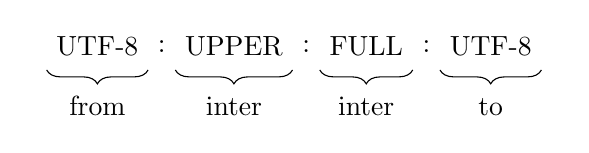
\begin{tikzpicture}[auto,node distance=0,on grid=false]
				    % Place nodes
				    \node (d0) {};
				    \node [right=of d0](from) {UTF-8};
				    \node [right=of from](d1) {:};
				    \node [right=of d1] (inter) {UPPER};
				    \node [right=of inter](d2) {:};
				    \node [right=of d2] (inter2) {FULL};
				    \node [right=of inter2](d3) {:};
				    \node [right=of d3] (to) {UTF-8};
				    \node [right=of to] (d4) {};			
					
					\draw [decorate,decoration={brace,amplitude=5pt,raise=3mm, mirror}]
	(d0) -- (d1) node [black,midway,yshift=-1cm] { from };
					
					\draw [decorate,decoration={brace,amplitude=5pt,raise=3mm, mirror}]
	(d1) -- (d2) node [black,midway,yshift=-1cm] { inter };
					
					\draw [decorate,decoration={brace,amplitude=5pt,raise=3mm, mirror}]
	(d2) -- (d3) node [black,midway,yshift=-1cm] { inter };
					
					\draw [decorate,decoration={brace,amplitude=5pt,raise=3mm, mirror}]
	(d3) -- (d4) node [black,midway,yshift=-1cm] { to };
				
				\end{tikzpicture}
				\caption{Conversion with multiple inter-mapping phases}
			\end{figure}

			\paragraph{}
			An \textbf{inter} phase can be used standalonely, mostly in programmatic way.
			\begin{figure}[H]
				\centering
				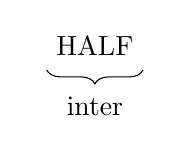
\begin{tikzpicture}[auto,node distance=0,on grid=false]

				    % Place nodes
				    \node (d0) {};
				    \node [right=of d0](inter) {HALF};
				    \node [right=of inter] (d1) {};
					
					\draw [decorate,decoration={brace,amplitude=5pt,raise=3mm, mirror}]
(d0)--(d1)  node  [black,midway,yshift=-1cm] { inter };
				\end{tikzpicture}
				\caption{Standalone inter-mapping phase}
			\end{figure}
			
			\paragraph{}
			Conversions can be cascaded with pipe symbol. In most cases it is equivalent to shell pipe unless the use of codecs manipulating flag (described in section 2.2).
			\begin{figure}[H]
				\centering
				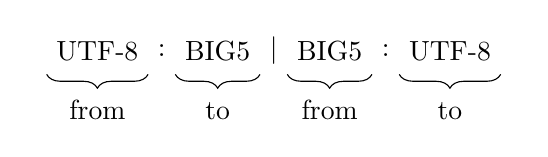
\begin{tikzpicture}[auto,node distance=0,on grid=false]
				    % Place nodes
				    \node (d0) {};
				    \node [right=of d0] (from) {UTF-8};
				    \node [right=of from] (d1) {:};
				    \node [right=of d1] (to) {BIG5};
				    \node [right=of to] (d2) {$|$};
				    \node [right=of d2] (from2) {BIG5};
				    \node [right=of from2](d3) {:};
				    \node [right=of d3](to2) {UTF-8};
				    \node [right=of to2] (d4) {};
					
					\draw [decorate,decoration={brace,amplitude=5pt,raise=3mm, mirror}] (d0) -- (d1) node [black,midway,yshift=-1cm] { from };
				
					\draw [decorate,decoration={brace,amplitude=5pt,raise=3mm, mirror}] (d1) -- (d2) node [black,midway,yshift=-1cm] { to };

					\draw [decorate,decoration={brace,amplitude=5pt,raise=3mm, mirror}] (d2) -- (d3) node [black,midway,yshift=-1cm] { from };

					\draw [decorate,decoration={brace,amplitude=5pt,raise=3mm, mirror}] (d3) -- (d4) node [black,midway,yshift=-1cm] { to };
				
				\end{tikzpicture}
				\caption{Cascaded conversions}
			\end{figure}
			\paragraph{}
			ASCII-compatible codecs are designed to exclude ASCII part and named as \_FOO, with alias FOO $\Rightarrow$ \_FOO,ASCII or ASCII,\_FOO.
		
		\subsection{Codecs \& Fallback}
			\paragraph{}
			A phase consists of one or more codecs, separated by comma. The latter codecs will be utilized if and only if the former codecs fail to consume the incoming data, once a codec finish its task, the first codec will be up again for upcoming data.
			\begin{figure}[H]
				\centering
				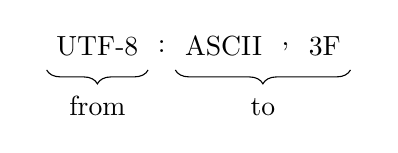
\begin{tikzpicture}[auto,node distance=0,on grid=false]
				    % Place nodes
				    \node (d0) {};
				    \node [right=of d0] (from) {UTF-8};
				    \node [right=of from] (d1) {:};
				    \node [right=of d1] (to) {ASCII};
				    \node [right=of to] (d2) {,};
				    \node [right=of d2] (from2) {3F};
				    \node [right=of from2] (d3) {};
					
					\draw [decorate,decoration={brace,amplitude=5pt,raise=3mm, mirror}] (d0) -- (d1) node [black,midway,yshift=-1cm] { from };
				
					\draw [decorate,decoration={brace,amplitude=5pt,raise=3mm, mirror}] (d1) -- (d3) node [black,midway,yshift=-1cm] { to };
				
				\end{tikzpicture}
				\caption{Fallback codec}
			\end{figure}
			
		\subsection{Codec argument}
			\paragraph{}
			Some codecs take arguments, after the hash symbol.
			\begin{figure}[H]
				\centering
				\begin{tikzpicture}[auto,node distance=0,on grid=false]
				    % Place nodes
				    \node (d0) {};
				    \node [right=of d0] (from) {UTF-8};
				    \node [right=of from] (d1) {:};
				    \node [right=of d1] (to) {ASCII};
				    \node [right=of to] (d2) {,};
				    \node [right=of d2] (to2) {ANY\#3F};
				    \node [right=of from2] (d3) {};
				
				\end{tikzpicture}
				\caption{Passing argument to codec}
			\end{figure}
			
			\paragraph{}
			Some codecs take arguments in key-value form. Argument name and value consist of numbers, alphabets, hyphen and underscore, binary data are represented in hexadecimal form. 
			\begin{figure}[H]
				\centering
				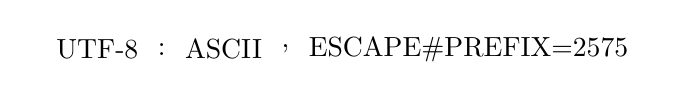
\begin{tikzpicture}[auto,node distance=0,on grid=false]
				    % Place nodes
				    \node (d0) {};
				    \node [right=of d0](from) {UTF-8};
				    \node [right=of from](d1) {:};
				    \node [right=of d1] (to) {ASCII};
				    \node [right=of to] (d2) {,};
				    \node [right=of d2] (to2) {ESCAPE\#PREFIX=2575};
				    \node [right=of to2] (d3) {};
				
				\end{tikzpicture}
				\caption{Passing argument to codec in key-value form}
			\end{figure}

			\paragraph{}
			Multiple arguments can be passed by being concatenated with ampersand.
			\begin{figure}[H]
				\centering
				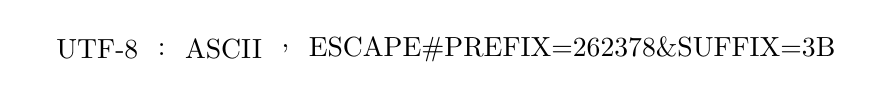
\begin{tikzpicture}[auto,node distance=0,on grid=false]
				    % Place nodes
				    \node (d0) {};
				    \node [right=of d0](from) {UTF-8};
				    \node [right=of from](d1) {:};
				    \node [right=of d1] (to) {ASCII};
				    \node [right=of to] (d2) {,};
				    \node [right=of d2] (to2) {ESCAPE\#PREFIX=262378\&SUFFIX=3B};
				    \node [right=of to2] (d3) {};
				
				\end{tikzpicture}
				\caption{Passing multiple arguments to codec}
			\end{figure}
			\paragraph{}
			List of data can be passed in dot-separated form.
			\begin{figure}[H]
				\centering
				
\begin{tikzpicture}[auto,node distance=0,on grid=false]
				    % Place nodes
				    \node (d0) {};
				    \node [right=of d0](from) {ANY\#013F.0121};
				    \node [right=of from](d1) {:};
				    \node [right=of d1] (to) {ASCII};
				    \node [right=of to] (d2) {};
				
				\end{tikzpicture}
				\caption{Data list}
			\end{figure}

	\section{Type \& Flag}
		\tikzstyle{data} = [rectangle, draw, text width=3em, text centered]
		\tikzstyle{type} = [rectangle, draw, fill=blue!30, text width=3em, text centered]
		\tikzstyle{flag} = [rectangle, fill=yellow, text width=3em, text centered]

		\subsection{Type}
			\paragraph{}
				A code point packet note its type at first byte.
				\begin{table}[H]
					\centering
					\begin{tabular}{|>{\columncolor{blue!30}}c | l | c | c|}
						\hline
						ID & Description & Provider(from) & Consumer(to)\\
						\hline
						00 & Bsdconv special characters & BSDCONV\_KEYWORD & BSDCONV\_KEYWORD\\
						01 & Unicode & Most decoder & Most encoder\\
						02 & CNS11643\footnotemark[1] & CNS11643 & CNS11643\\
						03 & Byte & BYTE; ESCAPE & BYTE; ESCAPE\#FOR=BYTE\\
						04 & Chinese components & inter/ZH\_DECOMP & inter/ZH\_COMP\\
						1B & ANSI control sequence & ANSI-CONTROL & -\\
						\hline
					\end{tabular}
					\caption{Types and its provider/consumer (just to name a few)}
				\end{table}
				\footnotetext[1]{As for the intersection of CNS11643 and Unicode, from/CNS11643 does conversion to unicode type if possible. Vice versa, to/CNS11643 does conversion from unicode type if possible.}
				\begin{figure}[H]
					\centering
					\begin{tikzpicture}[auto,node distance=0.5cm,on grid=false]
					    % Place nodes
					    \node (table){\begin{tabular}{|c|c|c|}
					    	\hline
					    	Entity & Unicode & UTF-8 Hex \\
					    	\hline
					    	\% & U+0025 & 25 \\
					    	A & U+0041 & 41 \\
					    	$\forall$ & U+2200 & E28880 \\
					    	\hline
						    \end{tabular}};
					    \node [below=1 of table,rectangle,draw] (input) {A$\forall$};
					    \node [below=0 of input] {Input (UTF-8 literal)};
					    \node [ellipse,draw,right=of input] (decoder) {ASCII,BYTE : ...};
					    \node [below=0 of decoder] {Decoder};
					    \node [rectangle,draw,right=of decoder] (internal) {
							\begin{tikzpicture}[node distance=3mm]
								\node [type](n0){01};
								\node [below=0 of n0,data](n1){41};
								\node [right=of n0,type](n2){03};
								\node [below=0 of n2,data](n3){E2};
								\node [right=of n2,type](n4){03};
								\node [below=0 of n4,data](n5){88};
								\node [right=of n4,type](n6){03};
								\node [below=0 of n6,data](n7){80};
								\draw [->] (n0) -- (n2);
								\draw [->] (n2) -- (n4);
								\draw [->] (n4) -- (n6);
							\end{tikzpicture}
					    };
					    \node [below=0 of internal] {Internal data};
					    \node [ellipse,draw,below=3cm of input] (encoder) {... : ASCII,ESCAPE};
					    \node [below=0 of encoder] {Encoder};
					    					    \node [rectangle,draw,right=of encoder] (internal2) {
							\begin{tikzpicture}[node distance=3mm]
								\node [data](n0){41};
								\node [above=0 of n0]{"A"};
								\node [right=of n0,data](n1){25};
								\node [below=0 of n1,data](n2){45};
								\node [below=0 of n2,data](n3){32};
								\node [above=0 of n1]{"\%E2"};
								\node [right=of n1,data](n4){25};
								\node [below=0 of n4,data](n5){38};
								\node [below=0 of n5,data](n6){38};
								\node [above=0 of n4]{"\%88"};
								\node [right=of n4,data](n7){25};
								\node [below=0 of n7,data](n8){38};
								\node [below=0 of n8,data](n9){30};
								\node [above=0 of n7]{"\%80"};
								\draw [->] (n0) -- (n1);
								\draw [->] (n1) -- (n4);
								\draw [->] (n4) -- (n7);
							\end{tikzpicture}
					    };
					    \node [below=0 of internal2] {Internal data};
					    \node [rectangle,draw,right=1 of internal2] (output) {A\%E2\%88\%80};
					    \node [below=0 of output] {Output (UTF-8 literal)};
					
						\draw [->] (input) -- (decoder);
						\draw [->] (decoder) -- (internal);
						\draw [->] (internal.east) -- ++ (0.5,0) -- ++ (0,-2) -| (encoder.north);
						\draw [->] (encoder) -- (internal2);
						\draw [->] (internal2) -- (output);
					\end{tikzpicture}
					\caption{Fallback \& Type}
				\end{figure}
		\clearpage
		
		\subsection{Flag}
			\paragraph{}
			A code point packet carries its own flags. Currently there are two types of flag, \textbf{FREE} and \textbf{MARK}. Flag \textbf{FREE} indicates that the packet buffer needs to be recycled or released, this is used only when programming is involved. Flag \textbf{MARK} is (currently only) added by codec to/PASS\#MARK and used by codec from/PASS\#UNMARK to identify which packets have already been decoded and needs to be passed through in \textbf{from} phase. 
			\paragraph{}
			The code point packets structure is retained, including flags, within cascaded conversions, but not for shell pipe. Figure 11 demonstrate the flow of conversion "ESCAPE:PASS\#MARK\&FOR=1,BYTE$|$PASS\#UNMARK,UTF-8:UTF-8".
				\begin{figure}[H]
					\centering
					\begin{tikzpicture}[auto,node distance=0.5cm,on grid=false]
					    % Place nodes
						\node (table){\begin{tabular}{|c|c|c|}
					    	\hline
					    	Entity & Unicode & UTF-8 Hex \\
					    	\hline
					    	$\alpha$ & U+03B1 & CEB1 \\
					    	$\beta$ & U+03B2 & CEB2 \\
					    	\hline
						    \end{tabular}};
					    \node [below=0.5cm of table,rectangle,draw] (input) {\%u03B1\%CE\%B2};
					    \node [below=0 of input] {Input (UTF-8 literal)};
					    \node [ellipse,draw,right=of input] (decoder) {ESCAPE : ...};
					    \node [below=0 of decoder] {Decoder};
					    \node [rectangle,draw,right=of decoder] (internal) {
							\begin{tikzpicture}[node distance=3mm]
								\node [type](n0){01};
								\node [below=0 of n0,data](n1){03};
								\node [below=0 of n1,data](n2){B1};
								\node [right=of n0,type](n3){03};
								\node [below=0 of n3,data](n4){CE};
								\node [right=of n3,type](n5){03};
								\node [below=0 of n5,data](n6){B2};
								\draw [->] (n0) -- (n3);
								\draw [->] (n3) -- (n5);
							\end{tikzpicture}
					    };
					    \node [below=0 of internal] {Internal data};
					    \node [ellipse,draw,below=2cm of input] (encoder) {... : PASS\#MARK\&FOR=1,BYTE};
					    \node [below=0 of encoder] {Encoder};
					    					    \node [rectangle,draw,right=1cm of encoder] (internal2) {
							\begin{tikzpicture}[node distance=3mm]
								\node [type](n0){01};
								\node [below=0 of n0,data](n1){03};
								\node [below=0 of n1,data](n2){B1};
								\node [below=0 of n2,flag]{MARK};
								\node [right=of n0,data](n3){CE};
								\node [right=of n3,data](n5){B2};
								\draw [->] (n0) -- (n3);
								\draw [->] (n3) -- (n5);
							\end{tikzpicture}
					    };
						\node [below=0 of internal2] {Internal data};
						\node [ellipse,draw,below=2cm of encoder] (decoder2) {PASS\#UNMARK,UTF-8 : ...};
						\node [below=0 of decoder2] {Decoder};
					    \node [rectangle,draw,right=of decoder2] (internal3) {
							\begin{tikzpicture}[node distance=3mm]
								\node [type](n0){01};
								\node [below=0 of n0,data](n1){03};
								\node [below=0 of n1,data](n2){B1};
								\node [right=of n0,type](n3){01};
								\node [below=0 of n3,data](n4){03};
								\node [below=0 of n4,data](n5){B2};
								\draw [->] (n0) -- (n3);
							\end{tikzpicture}
					    };
					    \node [below=0 of internal3] {Internal data};
						\node [ellipse,draw,right=of internal3] (encoder2) {... : UTF-8};
						\node [below=0 of encoder2] {Encoder};
					    \node [rectangle,draw,below=1.5cm of decoder2] (internal4) {
							\begin{tikzpicture}[node distance=3mm]
								\node [data](n0){CE};
								\node [below=0 of n0,data](n1){B1};
								\node [above=0 of n0]{"$\alpha$"};
								\node [right=of n0,data](n2){CE};
								\node [below=0 of n2,data](n3){B2};
								\node [above=0 of n2]{"$\beta$"};
								\draw [->] (n0) -- (n2);
							\end{tikzpicture}
					    };
					    \node [below=0 of internal4] {Internal data};
   					    \node [right=2cm of internal4,rectangle,draw] (output) {$\alpha\beta$};
					    \node [below=0 of output] {Output (UTF-8 literal)};

						\draw [->] (input) -- (decoder);
						\draw [->] (decoder) -- (internal);
						\draw [->] (internal.east) -- ++ (0.5,0) -- ++ (0,-1.35) -| (encoder.north);
						\draw [->] (encoder) -- (internal2);
						\draw [->] (internal2.east) -- ++ (1,0) -- ++ (0,-1.55) -| (decoder2.north);
						\draw [->] (decoder2) -- (internal3);
						\draw [->] (internal3) -- (encoder2);
						\draw [->] (encoder2.east)  -- ++ (0.5,0) -- ++ (0,-1.55) -|  (internal4.north);
						\draw [->] (internal4) -- (output);

					\end{tikzpicture}
					\caption{Flag, from/PASS \& to/PASS}
				\end{figure}
				
		\subsection{Helper codecs}
			\paragraph{}
			Codec from/bsdconv can be used to input internal data structure, and codec to/bsdconv\_stdout can be used to inspect type and flags.

	\section{C Programming guide}
		\subsection{Conversion instance lifecycle}
			\paragraph{}
				\begin{figure}[H]
					\centering
					\begin{tikzpicture}[auto,node distance=0.5cm,on grid=false]
						\tikzstyle{phase} = [rectangle, text centered]
						\node [phase](create){bsdconv\_create()};
						\node [phase,below=of create](init) {bsdconv\_init()};
						\node [phase,below=of init](parameter){set input/output parameters};
						\node [diamond,draw,below=of parameter](is_last){is last chunk};
						\node [phase,right=of is_last](flush){set flush flag};
						\node [phase,below=of is_last](conv){bsdconv()};
						\node [phase,below=of conv](output){collect output};
						\node [diamond,draw,below=of output](has_next){has next chunk};
						\node [phase,below=of has_next](destroy){bsdconv\_destroy()};
						\draw [->] (create) -- (init);
						\draw [->] (init) -- (parameter);
						\draw [->] (parameter) -- (is_last);
						\draw [->] (is_last) -- (flush)  node[midway,above]{yes};
						\draw [->] (is_last) -- (conv)  node[midway,right]{no};
						\draw [->] (conv) -- (output);
						\draw [->] (flush) -- (conv);
						\draw [->] (output) -- (has_next);
						\draw [->] (has_next) -- (destroy) node[near start,right]{no};
						\draw [->] (has_next.west) -- node[near start,above]{yes} ++ (-2, 0) |- (parameter.west) node[pos=0.25,left]{next chunk};
						\draw [->] (has_next.east) -- node[near start,above]{no} ++ (3, 0) |- (init.east) node[pos=0.25,right]{reuse instance};
					\end{tikzpicture}
					\caption{Conversion instance lifecycle}
				\end{figure}
		\clearpage
		\subsection{Skeleton}
			\begin{lstlisting}
#include <bsdconv.h>

bsdconv_instance *ins;
char *buf;
size_t len;
ins=bsdconv_create("UTF-8:UPSIDEDOWN:UTF-8");
bsdconv_init(ins);
do{
	buf=bsdconv_malloc(BUFSIZ);
	/*
	 * fill data into buf
	 * len=filled data length
	 */
	ins->input.data=buf;
	ins->input.len=len;
	ins->input.flags|=F_FREE;
	if(ins->input.len==0)
	{ // last chunk
		ins->flush=1;
	}
	/*
 	 * set output parameter (see section 3.3)
 	 */
	bsdconv(ins);
	/*
	 * collect output (see section 3.3)
	 */
}while(ins->flush==0);
bsdconv_destroy(ins);
			\end{lstlisting}
			\paragraph{}
				For chunked conversion, input buffer should be allocated for each input to prevent content change during conversion. Output buffer with flag \textbf{FREE} is safe to be reused.
		\subsection{Output mode}
			\begin{tabular}{|l|l|}
				\hline
				ins -$>$ output\_mode & Description \\
				\hline
				BSDCONV\_HOLD & Hold output in memory \\
				BSDCONV\_AUTOMALLOC & Return output buffer which should be free() after use\\
				BSDCONV\_PREMALLOCED & Fill output into given buffer\\
				BSDCONV\_FILE & Write output into (FILE *) stream file \\
				BSDCONV\_FD & Write output into (int) file descriptor \\
				BSDCONV\_NULL & Discard output \\
				\hline
			\end{tabular}
			\subsubsection{BSDCONV\_HOLD}
				\paragraph{}
				This is default output mode after bsdconv\_init(). Usually used with BSDCONV\_AUTOMALLOC or BSDCONV\_PREMALLOCED to get squeezed output.
			\subsubsection{BSDCONV\_AUTOMALLOC}
				\paragraph{}
				Output buffer will be allocated dynamically, the actual buffer size will be ins-$>$output.len + output content length, it is useful when you need to have terminating null byte.
			\subsubsection{BSDCONV\_PREMALLOCED}
				\paragraph{}
				If ins-$>$output.data is NULL, the total length of content to be output will be put to ins-$>$output.len, but output will still be hold in memory. Otherwise, bsdconv() will fill as much unfragmented data as possible within the buffer size limit specified at ins-$>$output.len.
			\subsubsection{BSDCONV\_FILE}
				\paragraph{}
				Output will be fwrite() to the given FILE * at ins-$>$output.data.
			\subsubsection{BSDCONV\_FD}
				\paragraph{}
				Output will be write() to the given (int) file descriptor at ins-$>$output.data. Casting to \textbf{intptr\_t} (defined in $<$stdint.h$>$) is needed to eliminate compiler warning.
			\subsubsection{BSDCONV\_NULL}
				\paragraph{}
				Output will be discard. This is usually used with evaluating conversion (see section 3.4).

		\subsection{Counters}
			Counters are listed in ins-$>$counters in linked-list with following structure.
			\begin{lstlisting}
struct bsdconv_counter_entry{
	char *key;
	counter_t val;
	struct bsdconv_counter_entry *next;
};
			\end{lstlisting}
			IERR and OERR are mandatory error counters.
			\newpage\noindent
			There are two API to get/reset counter(s):
			\begin{lstlisting}
bsdconv_counter_t * bsdconv_counter(char *name);
			\end{lstlisting}
			Return the pointer to the counter value. bsdconv\_counter\_t is currently defined as size\_t.
			\begin{lstlisting}
void bsdconv_counter_reset(char *name);
			\end{lstlisting}
			Reset the specified counter, if name is NULL, all counters are reset.
		\subsection{Memory pool issue}
			\paragraph{}
			In case libbsdconv and your program uses different memory pools, bsdconv\_malloc() and bsdconv\_free() should be used to replace malloc() and free().
\end{document}